\chapter{Document Age Prediction Model}
\label{ch:doc}

\definecolor{eclipseStrings}{RGB}{42,0.0,255}
\definecolor{eclipseKeywords}{RGB}{127,0,85}
\colorlet{numb}{magenta!60!black}
\colorlet{punct}{red!60!black}
\definecolor{delim}{RGB}{20,105,176}

\lstset{
  basicstyle=\ttfamily,
  columns=fullflexible,
  showstringspaces=false,
  commentstyle=\color{gray}\upshape,
  breaklines=true
}
\lstdefinelanguage{json}
{
%     morestring=[b]",
%     morestring=[d]'
  commentstyle=\color{eclipseStrings}, % style of comment
  stringstyle=\color{eclipseKeywords}, % style of strings
  numbers=left,
  frame=lines,
  %backgroundcolor=\color{gray}, %only if you like
  string=[s]{"}{"},
  comment=[l]{:\ "},
  morecomment=[l]{:"},
  literate=
  *{0}{{{\color{numb}0}}}{1}
  {1}{{{\color{numb}1}}}{1}
  {2}{{{\color{numb}2}}}{1}
  {3}{{{\color{numb}3}}}{1}
  {4}{{{\color{numb}4}}}{1}
  {5}{{{\color{numb}5}}}{1}
  {6}{{{\color{numb}6}}}{1}
  {7}{{{\color{numb}7}}}{1}
  {8}{{{\color{numb}8}}}{1}
  {9}{{{\color{numb}9}}}{1}
  {:}{{{\color{punct}{:}}}}{1}
  {,}{{{\color{punct}{,}}}}{1}
  {\{}{{{\color{delim}{\{}}}}{1}
  {\}}{{{\color{delim}{\}}}}}{1}
  {[}{{{\color{delim}{[}}}}{1}
  {]}{{{\color{delim}{]}}}}{1},
}

In order to model how recent a document is, we try to predict the time the current content was last updated. Given that information, we can define the document age as:
\[ documentAge = currentTime - documentLastUpdateTime \]
Here, $currentTime$ is the time when we are observing the document, for example, at query issue time.

If we know the last update time of a document, it is trivial to calculate the document age on the fly. For example, in the case of news search, it is almost always the case that we are provided with a publication time and we can simply use it as a feature, as seen in \citep{dakka2012answering}. Moreover, \citet{spitz2018predicting} have shown that, for news articles, we can also take advantage of the citation network, or the inbound and outbound links in the articles.

However, as we are focusing on documents on the Web in general, we cannot assume that we have this information readily available. To this end, we developed a machine-learned model to predict the last update time of a document.

We approach this as a supervised regression problem, so we first obtain a labeled set of documents to serve as ground truth. We extract features from the content of the document which indicate when the document was last updated, and learn and evaluate a machine learning model. We explain how we compile the ground truth in the next section.

\section{Ground Truth Creation}
We create a ground truth set for a random sample of 5K documents from our document index. Instead of manually annotating the time a document was last updated, we infer it automatically by querying the Memgator web service.\footnote{\url{http://memgator.cs.odu.edu/}.} As described by \citet{salaheldeen2013carbon}, this service can be used for navigating between the current and the past web. It provides a list of \textit{mementos}, or timestamps, when the document was changed. We note that a memento timestamp is the time of capture at the web archive, which might not entirely align with the actual update time of the document. However, we deemed this approximation good enough for our purposes.

For a given URI, the service returns a list of timestamps, ordered from oldest to newest, when there was an update to the Web page. Figure \ref{code:memgator} shows an example of a request and response from the service. The list of mementos is shortened for readability.

\begin{lstlisting}[language=json,firstnumber=1,caption=Example of a request to and response from the Memgator web service., label=code:memgator]]
curl "https://memgator.cs.odu.edu/timemap/json/www.ntent.com"
{
  original_uri: "http://www.ntent.com",
  self: "https://memgator.cs.odu.edu/timemap/json/www.ntent.com",
  mementos: {
    list: [
      {
        datetime: "2000-04-08T22:25:51Z",
        uri: "http://web.archive.org/web/20000408222551/www.ntent.com:80/"
      },
      (...)
      {
        datetime: "2018-06-14T23:55:54Z",
        uri: "http://web.archive.org/web/20180614235554/www.ntent.com/"
      }
  ]
    first: {
        datetime: "2000-04-08T22:25:51Z",
        uri: "http://web.archive.org/web/20000408222551/www.ntent.com:80/"
    },
    last: {
        datetime: "2018-06-14T23:55:54Z",
        uri: "http://web.archive.org/web/20180614235554/www.ntent.com/"
    }
  }
\end{lstlisting}

A naïve approach would be to take the \texttt{last} field from the JSON, signifying the time of the last recorded change. However, when dealing with documents on the Web, it is often the case that an update is not actually a content update, but a page maintenance update. In other words, the change in document content is negligible and we do not want to capture such \textit{near-duplicates}.

To make sure we are capturing actual content updates, we traverse the list of last updates in reverse, from the latest to oldest timestamp, and compare the current document content to the previous one. If the similarity is above a certain threshold ($t$ = 90\%), we discard the update and keep going back in time. We compute the similarity between two documents by \textit{shingling} them \citep{broder1997resemblance}.

Shingling is a technique used in information retrieval to detect near-duplicate documents. Given a positive integer $k$ and a sequence of terms in a document $d$, we define the $k$-shingles of $d$ to be the set of all consecutive sequences of $k$ terms in $d$. Let $S(d_j)$ denote the set of shingles of document $d_j$. For example, for $d$ = \textit{Barcelona is the capital of Catalonia}, and $k = 3$, the shingles are \{(Barcelona, is, the), (is, the, capital), (the, capital, of), (capital, of, Catalonia)\}. We then produce an MD5 hash of each shingle, sort them alphabetically, and take the first $N$ shingles as a set. We denote this as $S(d_j)$. We compute the Jaccard coefficient to measure the degree of overlap between the sets $S(d_1)$ and $S(d_2)$ as:
\[ J(S(d_1),S(d_2)) = \frac{\vert S(d_1) \cap S(d_2)\vert}{\vert S(d_1) \cup S(d_2)\vert}. \]

\noindent If $J(S(d_1),S(d_2)) < 0.90$, the documents are assumed to be distinct.

Finally, the ground truth dataset consists of $5248$ documents, where each document object contains the following fields:
\begin{enumerate}
	\item \texttt{URL.} The full URL of a document, also a unique identifier of a document.
	\item \texttt{FullHTML.} The full HTML content retrieved by the crawler, without any preprocessing.
    \item \texttt{ContentHTML.} The content of the document after boilerplate removal was performed. This does not contain JavaScript blocks, CSS, and such.
    \item \texttt{DocumentLastUpdateTime.} The target variable, obtained using the aforementioned technique, expressed as Unix time.\footnote{Unix time is the number of seconds that have elapsed since January 1, 1970.}
\end{enumerate}

\section{Feature Extraction}
We extract features from the URL and the content of the document. For the content, we process both the full HTML of the document (before boilerplate removal), and from the clean HTML (after boilerplate removal). Table \ref{tb:dataset-doc} shows the statistics of the documents from our ground truth. The average length of the raw document HTML is ten times longer than the clean one. Although some of this is due to the HTML format (e.g., tags and attributes), there is still a lot of noisy content that could be used to extract features indicative of the document's last modification date. Therefore, we choose to process both versions of the document, and have both groups of extracted features in the resulting feature vector.

\begin{table}[h!]
\centering
\caption{Ground truth dataset statistics.}
\label{tb:dataset-doc}
\begin{tabular}{@{}cccc@{}}
\toprule
Number of documents & Average FullHTML size & Average ContentHTML size &  \\ \midrule
5248 & 108054 characters & 10961 characters &  \\ \bottomrule
\end{tabular}
\end{table}

First, we develop a pattern-matching solution to extract any mention of dates. A comprehensive list of supported date formats is shown in Table \ref{tb:dates}.

\begin{table}[!htbp]
\centering
\caption{Date formats supported in regular expressions.}
\label{tb:dates}
\begin{tabular}{@{}ll|ll@{}}
\toprule
Date format & Example date & Date format & Example date \\ \midrule
dd/mm/yy & 27/05/93 & yy-mmm-dd & 93-Aug-27 \\
dd/mm/yyyy & 27/05/1993 & yy-mmmm-dd & 93-August-27 \\
d/m/yy & 5/5/93 & mm/dd/yy & 05/27/93 \\
d/m/yyyy & 5/5/1993 & mm/dd/yyyy & 05/27/1993 \\
dd-mmm-yy & 27-Aug-93 & mmm-dd-yy & Aug-27-93 \\
dd-mmm-yyyy & 27-Aug-1993 & mmm-dd-yyyy & Aug-27-1993 \\
d-mmmm-yy & 27-August-93 & mmmm dd, yyyy & August 27, 1993 \\
d-mmmm-yyyy & 27-August-1993 & dd mmmm yyyy & 27 August 1993 \\
yy/mm/dd & 93/05/27 & mmm yyyy & Aug 1993 \\
yyyy/mm/dd & 1993/05/27 & mmmm, yyyy & August, 1993 \\
yyyy-mm-dd & 1993-05-27 & yyyy & 1993 \\ \bottomrule
\end{tabular}
\end{table}

We denote the features that capture dates as \texttt{timestamp features}. When extracting timestamps containing uncertainty of the exact date, we take the approach as \citet{berberich2010language}. More specifically, we support both Americanized date formats (first month, then day) and standardized (first day, then month). We use several regular expressions to capture different date formats, transform all dates to a standardized format \texttt{YYYY-MM-DD}, then convert the extracted dates to Unix time. Moreover, since we aim to predict the last update time on a year-month scale, we set the day field to the 15th of the month.

Apart from the \texttt{timestamp features}, we also extract features from specific \texttt{<meta>} tags, called \texttt{meta tag features}, and the \texttt{jQuery version feature}. The total number of features is 20, where each feature value is expressed as Unix time. The list of features is shown in Table \ref{tb:features}.

\begin{table}[]
\centering
\caption{List of features.}
\label{tb:features}
\begin{tabular}{@{}cl@{}}
\toprule
Feature index & Feature name                                     \\ \midrule
1             & TimestampFeatures\_FullHtml\_MinTimestamp        \\
2             & TimestampFeatures\_FullHtml\_MaxTimestamp        \\
3             & TimestampFeatures\_FullHtml\_AvgTimestamp        \\
4             & TimestampFeatures\_FullHtml\_FirstTimestamp      \\
5             & TimestampFeatures\_FullHtml\_LastTimestamp       \\
6             & TimestampFeatures\_FullHtml\_MostCommonYear      \\
7             & TimestampFeatures\_FullHtml\_MostCommonYearMonth \\
8             & TimestampFeatures\_Html\_MinTimestamp            \\
9             & TimestampFeatures\_Html\_MaxTimestamp            \\
10            & TimestampFeatures\_Html\_AvgTimestamp            \\
11            & TimestampFeatures\_Html\_FirstTimestamp          \\
12            & TimestampFeatures\_Html\_LastTimestamp           \\
13            & TimestampFeatures\_Html\_MostCommonYear          \\
14            & TimestampFeatures\_Html\_MostCommonYearMonth     \\
15            & MetaTagFeatures\_FullHtml\_LastModified                   \\
16            & MetaTagFeatures\_FullHtml\_Copyright                      \\
17            & MetaTagFeatures\_FullHtml\_DCDateIssued                   \\
18            & MetaTagFeatures\_FullHtml\_DCTermsModified                \\
19            & JQueryVersion                                    \\
20            & TimestampFeatures\_Url                                     \\ \bottomrule
\end{tabular}
\end{table}

\subsection{Timestamp Features}
We extract \texttt{timestamp features} from the full HTML of the document (pre-boilerplate removal), the clean HTML (post-boilerplate removal), and document URL. We want to be able to predict the last update time of a document on a monthly scale, so we only store the year and month of retrieved timestamps, whereas we always set the day value to the 15th.

The \texttt{timestamp features} are the following:
\begin{itemize}
	\item \texttt{MinTimestamp:} the minimal timestamp mentioned;
    \item \texttt{MaxTimestamp:} the maximal timestamp mentioned;
    \item \texttt{AvgTimestamp:} the average timestamp mentioned;
    \item \texttt{FirstTimestamp:} the first timestamp mentioned;
    \item \texttt{LastTimestamp:} the last timestamp mentioned;
    \item \texttt{MostCommonYear:} the most commonly mentioned year, converted to June 15th of that year;
    \item \texttt{MostCommonYearMonth:} the most commonly mentioned year and month, converted to the 15th of that month.
\end{itemize}

We also extract any timestamps that are mentioned in the URL and model it as a separate feature.

\subsection{Other Features}
For the \texttt{meta tag features}, we capture four different tag types:

\begin{lstlisting}[language=json]
<meta name="Last-Modified" content="2017-06-05 11:21:43">
<meta name="copyright" content="Copyright (c) 2017 ABC News Internet Ventures">
<meta name="dcterms.modified" content="2007-12-20 11:17:23">
<meta property="DC.date.issued" content="2017-04-27T08:00:40-04:00">
\end{lstlisting}

Lastly, for the \texttt{jQuery feature}, we precomputed a lookup table of release dates of different jQuery versions.\footnote{\url{https://gist.github.com/0xdevalias/8e558f4ed452ec54880e8b8445d13e28 }.} Often times, documents include a snippet referencing the minimum jQuery version, such as:
\begin{lstlisting}[language=json]
<script src="https://ajax.googleapis.com/ajax/libs/jquery/1.7.2/jquery.min.js"></script>
\end{lstlisting}

If there is a mention of a jQuery version number in the full HTML, we set the \texttt{jQuery feature} value as the release date of that version.

\section{Model Training}
% what is a train instance, framework used, feature importance
We use Gradient Boosted Regression Trees (GBRT) as the model. Gradient boosting is a machine learning technique where the prediction model is an ensemble of weak prediction models, in this case decision trees. The idea of gradient boosting was first introduced by \citet{breiman1997arcing}. Later, \citet{friedman2001greedy} introduced improvements to the boosting algorithms.

Decision trees were suitable for this problem, as they are easy to interpret, they require little data preparation, and have built-in feature selection. We use XGBoost (eXtreme Gradient Boosting), introduced by \citet{chen2016xgboost}, an open-source parallel gradient boosting library to train and evaluate the model.

As mentioned earlier, we have a total of 20 features, where each feature value is Unix time. Each training instance is of the \texttt{LibSVM data format}:\footnote{\url{https://www.csie.ntu.edu.tw/~cjlin/libsvm/}.}
\[ \texttt{<label> <index\_1>:<value\_1> ... <index\_N>:<value\_N>} \]

Here, \texttt{<label>} is the target value, expressed in Unix time, and the rest of the fields model the feature index and value, respectively.

To investigate which features are more useful than others, we plot the feature importance scores, as seen in Figure \ref{fig:fscores}. By looking at the feature overview in Table \ref{tb:features}, we can see that the first five features, \texttt{timestamp features} retrieved from the full HTML content, are the most important, followed by \texttt{timestamp features} retrieved from the clean HTML. The worst-performing group of features are the \texttt{meta tag features}, due to the fact that these attributes are seldom included in documents in our collection. The same applies for the \texttt{jQuery version feature}, which, although very indicative of the document publication date, was rarely present in our document set.

\begin{figure}
  \centering
  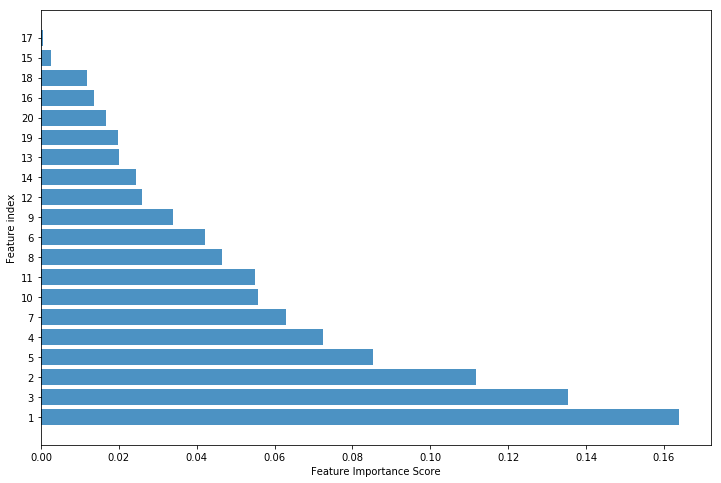
\includegraphics[width=\linewidth]{img/doc_f_importance.png}
  \caption{Feature importance scores of the document age prediction model.}
  \label{fig:fscores}
\end{figure}
% plotted in queries.ipynb

% add/expand discussion of features, how often they're present, why we chose them etc.

\section{Evaluation}
\label{sec:docparams}
For training the model, we split the input set into train and validation sets in the 70:30 ratio. We then proceeded to grid search the hyper-parameters of the model using a 5-fold cross-validation. Listing~\ref{param-doc} shows which hyper-parameters are tuned.

\begin{lstlisting}[language=json,caption=Hyper-parameter tuning for the document age model.,label=param-doc]
'max_depth': [4, 6, 8, 10], (best = 4)
'min_child_weight': [0, 1, 2], (best = 0)
'gamma': [0.0, 0.1, 0.2, 0.3], (best = 0.0)
'subsample': [0.6, 0.8, 1.0], (best = 1.0)
'colsample_bytree': [0.6, 0.8, 1.0], (best = 0.6)
'learning_rate': [0.01, 0.03, 0.1, 0.2, 0.3], (best = 0.01)
'n_estimators': [100, 500, 1000, 5000],  (best = 1000)
\end{lstlisting}

%  Best hyperparameters:
% {'colsample_bytree': 0.6, 'learning_rate': 0.01, 'min_child_weight': 0, 'n_estimators': 1000, 'subsample': 1.0, 'max_depth': 4, 'gamma': 0.0}
% RMSE (train) 32026382.3785 or 3.202e+07
% RMSE (test): 3.596e+07

Parameter \texttt{max\_depth} is the maximum depth of a tree, and increasing this value will make the model more complex and likely to overfit. Parameter \texttt{min\_child\_weight} is the minimum sum of instance weight needed in a child to continue further partitioning. The larger, the more conservative the model. Parameter \texttt{gamma} is the minimum loss reduction required to make a further partition on a leaf node of the tree. The larger, the more conservative the model. Parameter \texttt{subsample} is the ratio of training instances to subsample. Setting it to 0.5 means that XGBoost randomly collects half of the data instances to grow trees and this will prevent overfitting. Parameter \texttt{colsample\_bytree} is the subsample ratio of columns when constructing each tree. Parameter \texttt{learning\_rate} is the step size shrinkage used in the update phase to prevent overfitting. Parameter \texttt{n\_estimators} is the number of trees to construct.

The training of the model took 23 hours on a machine with CentOS 7.5.1804, 16 GB of RAM, and 8 Intel(R) Xeon(R) CPU E5-2660 v3 @ 2.60GHz CPUs. The model was trained by minimizing the root mean squared error (RMSE) of the difference between the predicted Unix time value and the value from the ground truth. 

The results on the train and test sets are shown in Table \ref{tb:docclass}. To provide a better intuition for the results, the epoch timestamp (or Unix time) of \texttt{26 June 2018} is $1529971200$. Moreover, an RMSE value of $3e+07$ is equivalent to \texttt{14 December 1970}. Since Unix time is defined as the number of seconds since \texttt{1 January 1970}, we can conclude that the model's predictions are accurate within a year.

\begin{table}[h!]
\centering
\caption{Document age prediction model evaluation.}
\label{tb:docclass}
\begin{tabular}{@{}ll@{}}
\toprule
RMSE train & RMSE test \\ \midrule
3.202e+07  & 3.596e+07 \\ \bottomrule
\end{tabular}
\end{table}

To gain insight into how our model is performing, we plot two different learning curves. The first learning curve, shown in Figure \ref{fig:doc-curve1}, shows the model performance based on the number of training rounds. We run a 5-fold cross-validation on different subsets of training instances. We expect to see an increase in the error on the training set, as we increase the number of training instances. This is because the model is likely to overfit and predict well when given a smaller number of training instances. However, as the model is trained on more data, it manages to fit better the validation set. Thus, the validation error decreases. Based on this graph, it looks like we could benefit from adding more training instances, and still not be at risk of overfitting the model.

The second learning curve is shown in Figure \ref{fig:doc-curve2}. Here, we examine the model's performance based on the number of training rounds. We notice that both the training and validation error reduce rapidly. Nevertheless, the validation error does not reduce significantly after 400 rounds. If we wanted to reduce the time and computational power necessary to train the model, this graph shows we can stop training after 400 rounds, since no significant improvement is observed after that point. Note, however, that we trained the model with setting the configuration parameter \texttt{early\_stopping\_rounds} to 50, which means there was a reduction in validation error after all.

\begin{figure}
\centering
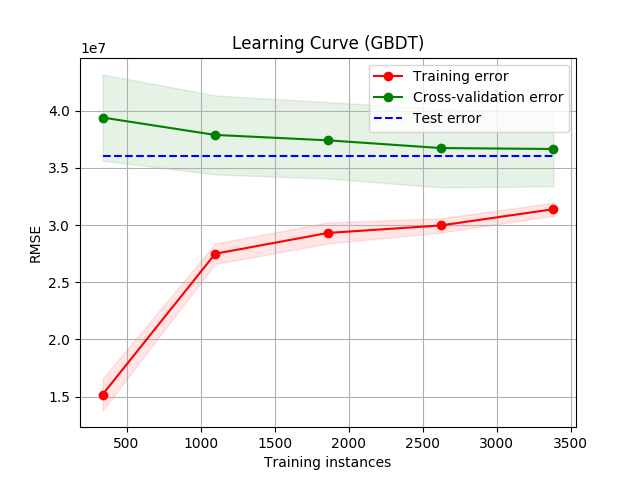
\includegraphics[width=0.8\linewidth]{img/doc_learning_curve.png}
\caption{Learning curve of the document age prediction model based on the number of training instances.}
\label{fig:doc-curve1}
\end{figure}

\begin{figure}
\centering
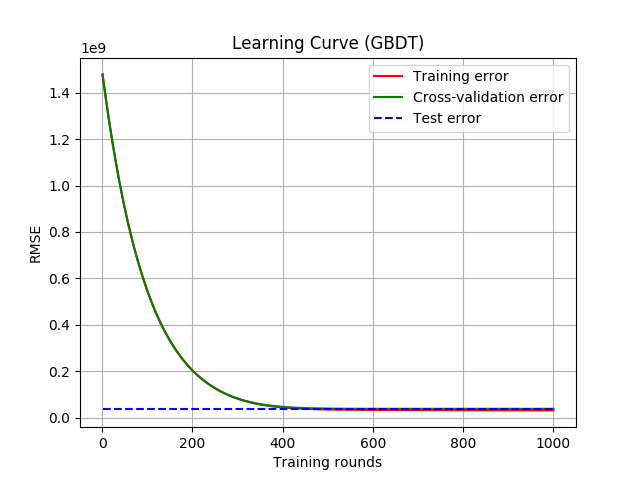
\includegraphics[width=0.8\linewidth]{img/doc_learning_curve2.png}
\caption{Learning curve of the document age prediction model based on the number of training rounds.}
\label{fig:doc-curve2}
\end{figure}

